\section{HERMES and COMPASS results of Leading-Order  purity method }
The HERMES~\cite{Airapetian:2004zf} and COMPASS~\cite{Alekseev:2010ub} analysis explicitly assumed the $x-z$ naive separation  of Eq.~\ref{eq:fact}
at the leading order, the asymmetries are related to the parton polarizations
through linear relations as: 
\begin{equation}
A_{1N}^h(x,Q^2,z) =  
{ \sum_f  e_f^2 \Delta q_f(x,Q^2) \cdot D_f^{h}(z, Q^2) 
\over \sum_f e_f^2 q_f(x,Q^2) \cdot D_f^{h}(z,Q^2) }.
\label{Eq:a1h2}
\end{equation} 

The HERMES and COMPASS analysis used the 
``purity method'' to achieve leading order 
flavor decomposition~\cite{purity}. In Eq.~\ref{Eq:a1h2},
a ``purity matrix'' ${\cal P}_f^h(x,Q^2,z)$ was defined such that:

\begin{equation}
A_{1N}^h(x,Q^2,z) \equiv \sum_f {\cal P}_f^h(x,Q^2,z) \cdot 
{\Delta q_f(x,Q^2) \over q_f(x,Q^2)},
\label{Eq:a1pur}
\end{equation}  
where
\begin{equation}
{\cal P}_f^h(x)= { e_f^2  q_f(x) \int dz  D_f^{h}(z) \over \sum_{i}  e_{i}^2  
q_{i}(x) \int dz  D_{i}^{h}(z) },
\end{equation}  
and the explicit $Q^2$ notation has been omitted for simplicity.
The ``purity method'' integrates over all the experimentally allowed $z$-range such 
that SIDIS events are included as much as possible to improve statistical accuracy.
The exact values of ${\cal P}_f^h(x,Q^2,z)$ in the HERMES analysis were obtained through a detailed
Monte Carlo simulation which was based on the Lund fragmentation model~\cite{lund} 
and take into account the experimental phase space and detector efficiencies. The parameters 
used in the fragmentation model were fine-tuned in order to reproduce the measured hadron yields. 
 
Integrating over hadrons with $0.2<z<0.8$, HERMES extracted five flavor quark polarizations:
\begin{equation}
\vec Q = \left( x \Delta u , x \Delta d ,  x \Delta \bar{u},  x \Delta \bar{d},  
x \Delta {s} \right),
\end{equation}  
from a data base of measured double-spin asymmetries
\begin{equation}
 \vec A= \left( A_{1p}^{\pi^+}, A_{1p}^{\pi^-}, A_{1d}^{\pi^+}, A_{1d}^{\pi^-},
  A_{1d}^{K^+}, A_{1d}^{K^-}, A_{1p}, A_{1d}\right)
\end{equation}  
by solving the relations of $\vec A= {\cal P}_f^h(x)  \cdot \vec Q$. The HERMES data on 
proton and deuteron asymmetries~\cite{hermes2002}
are shown in Fig.~\ref{fig:ahermesp} and~\ref{fig:ahermesd} 
in comparison with the SMC data~\cite{smc1998}. 
%The ratio of $\Delta q/q$ for each flavor 
%from the purity method is shown in Fig.~\ref{fig:polqq}
%-------------------------------------------------------------------------------
\begin{figure}[htbp]
  \centering
    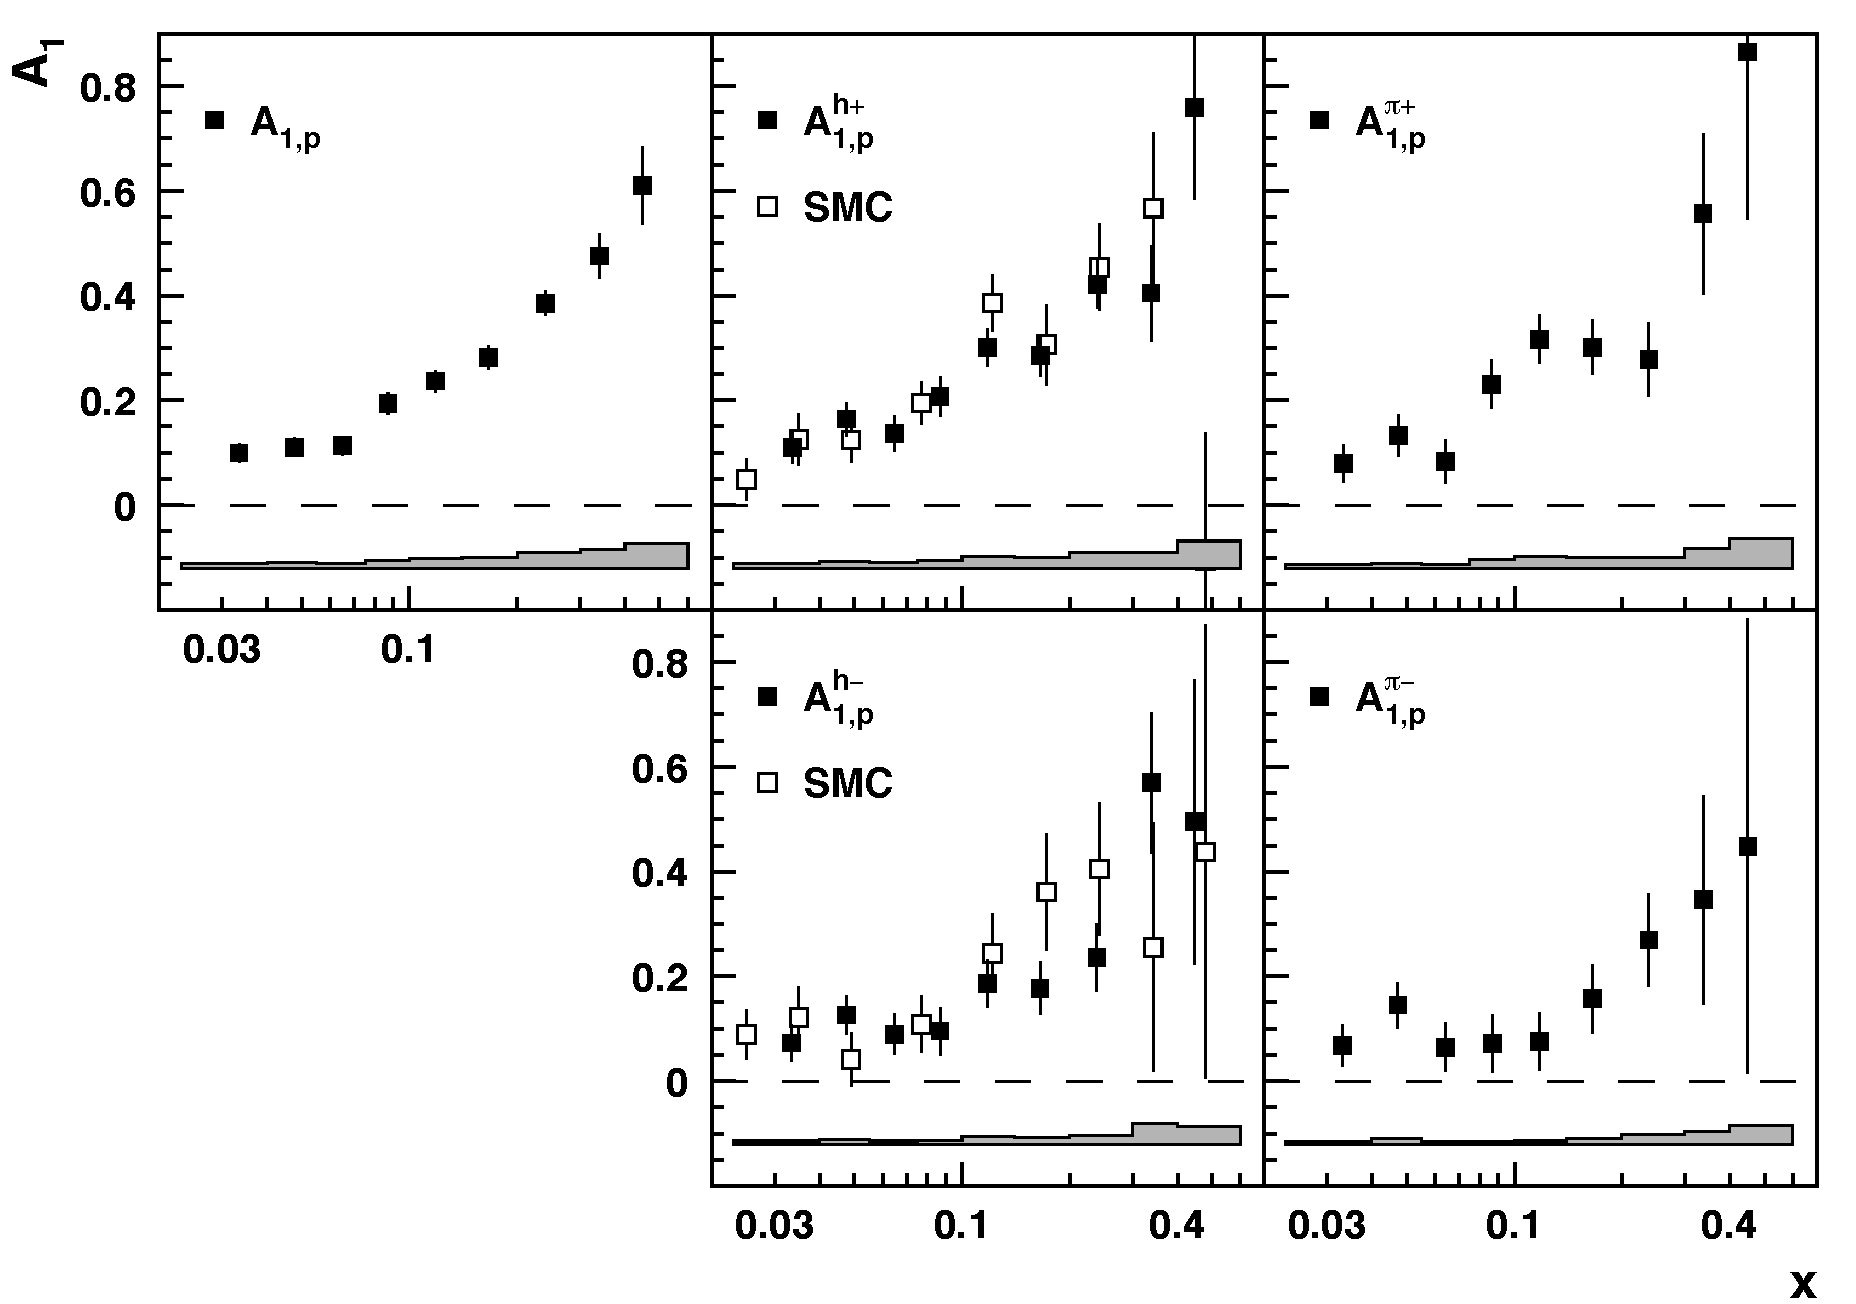
\includegraphics[width=0.90\linewidth]{./figs_xj/hermes_prd_A1p-all.pdf}
\caption{\label{fig:ahermesp} The double-spin asymmetries on proton   $A_{1p}^h$ form HERMES~\protect\cite{Airapetian:2004zf}
 and SMC~\protect\cite{Adeva:1997qz}. 
}
\end{figure}
%-------------------------------------------------------------------------------
%-------------------------------------------------------------------------------
\begin{figure}[htbp]
  \centering
    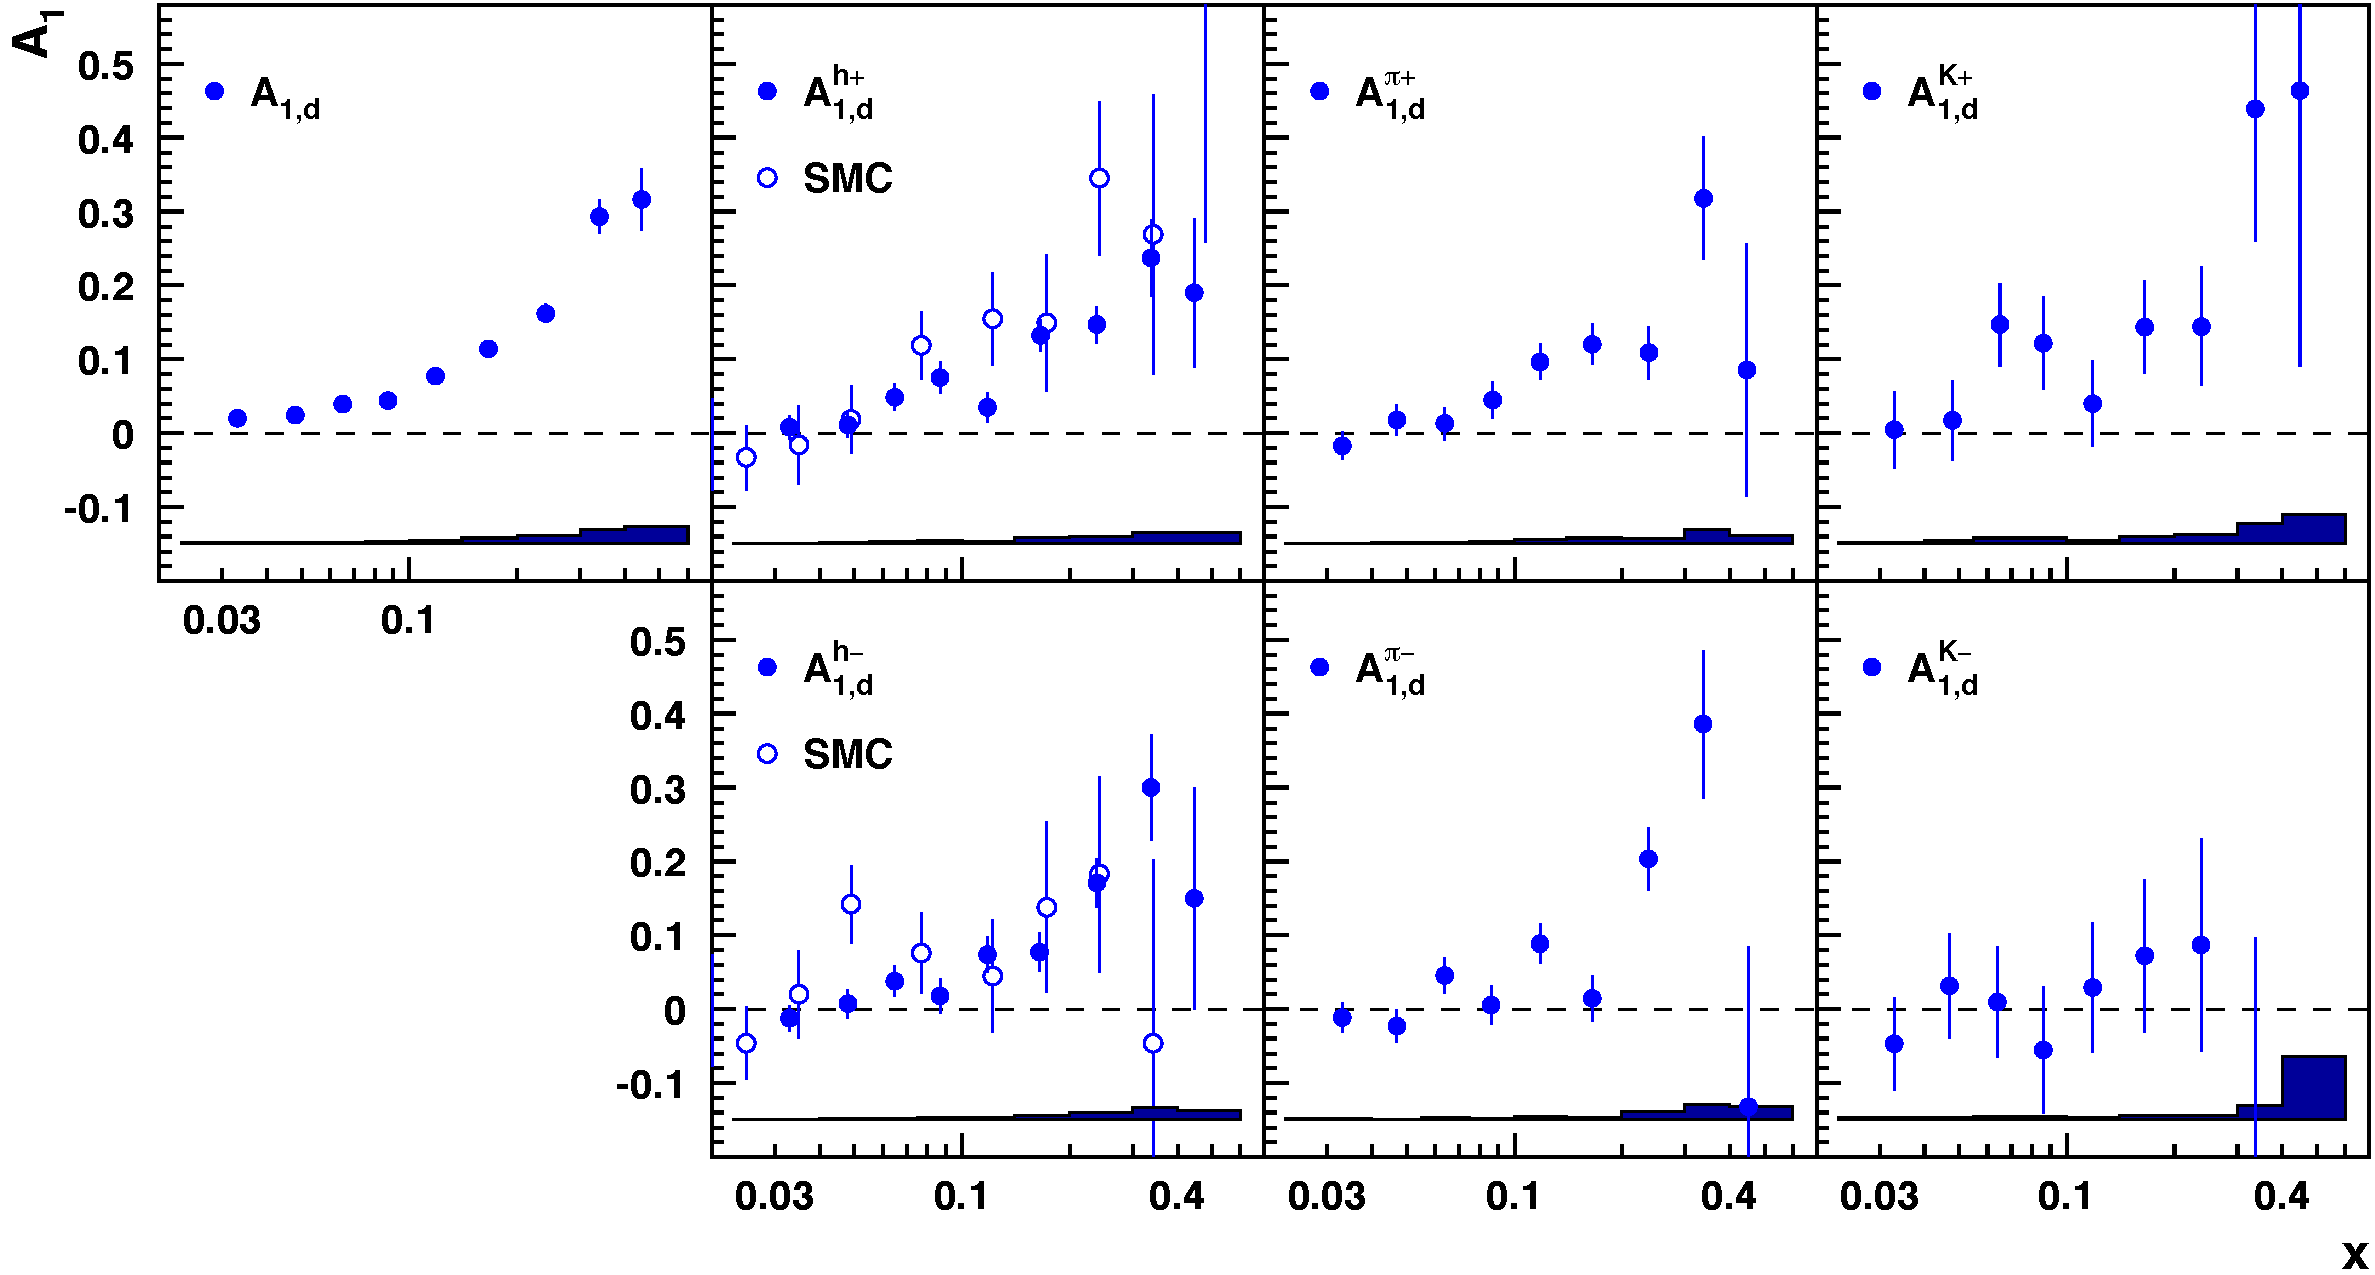
\includegraphics[width=0.90\linewidth]{./figs_xj/hermes_prd_A1d-all_color.pdf}
\caption{\label{fig:ahermesd} The double-spin asymmetries on deuteron 
 $A_{1d}^h$ form HERMES~\protect\cite{Airapetian:2004zf}
 and SMC~\protect\cite{Adeva:1997qz}. 
}
\end{figure}
%-------------------------------------------------------------------------------


An independent effort of flavor decomposition using the \lo Christova-Leader method
has also been carried out in the HERMES analysis~\cite{hermesthesis}, although not presented in the
published data.  However, due to the unfavorable $\pi^-/\pi^+$ ratio at higher-$x$ bins in HERMES,
the statistical uncertainties of the Christova-Leader method are rather large compared to
that of the purity method, as shown in Fig.~\ref{fig:hermescl} 
%-------------------------------------------------------------------------------
\begin{figure}[htbp]
  \centering
    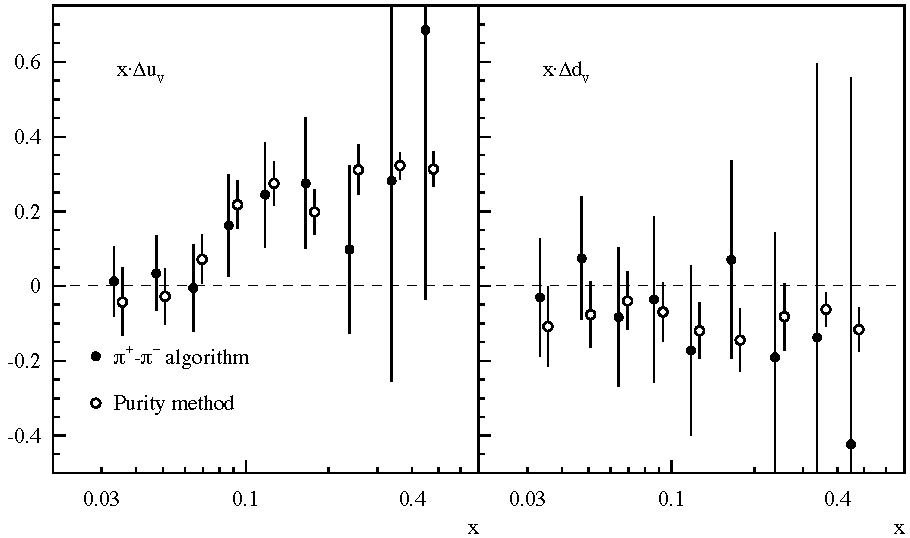
\includegraphics[width=0.90\linewidth]{./figs_xj/hermes_thesis_cl_xuvdv-pions.pdf}
\caption{\label{fig:hermescl}
Statistical error comparison of the HERMES purity method (open circles) with the HERMES 
Christova-Leader method analysis~\protect\cite{hermesthesis} (solid circles). 
}
\end{figure}
%-------------------------------------------------------------------------------

Recently, the COMPASS experiment~\cite{compass2007} released the results of $A_d^{h^+}$ and $A_d^{h^-}$, identified charged hardon asymmetries off a deuteron target, with improved statistical precisions at lower-$x$ region. The asymmetry results are shown in Fig.~\ref{fig:compass1}.   
%-------------------------------------------------------------------------------
\begin{figure}[tbhp]
  \centering
    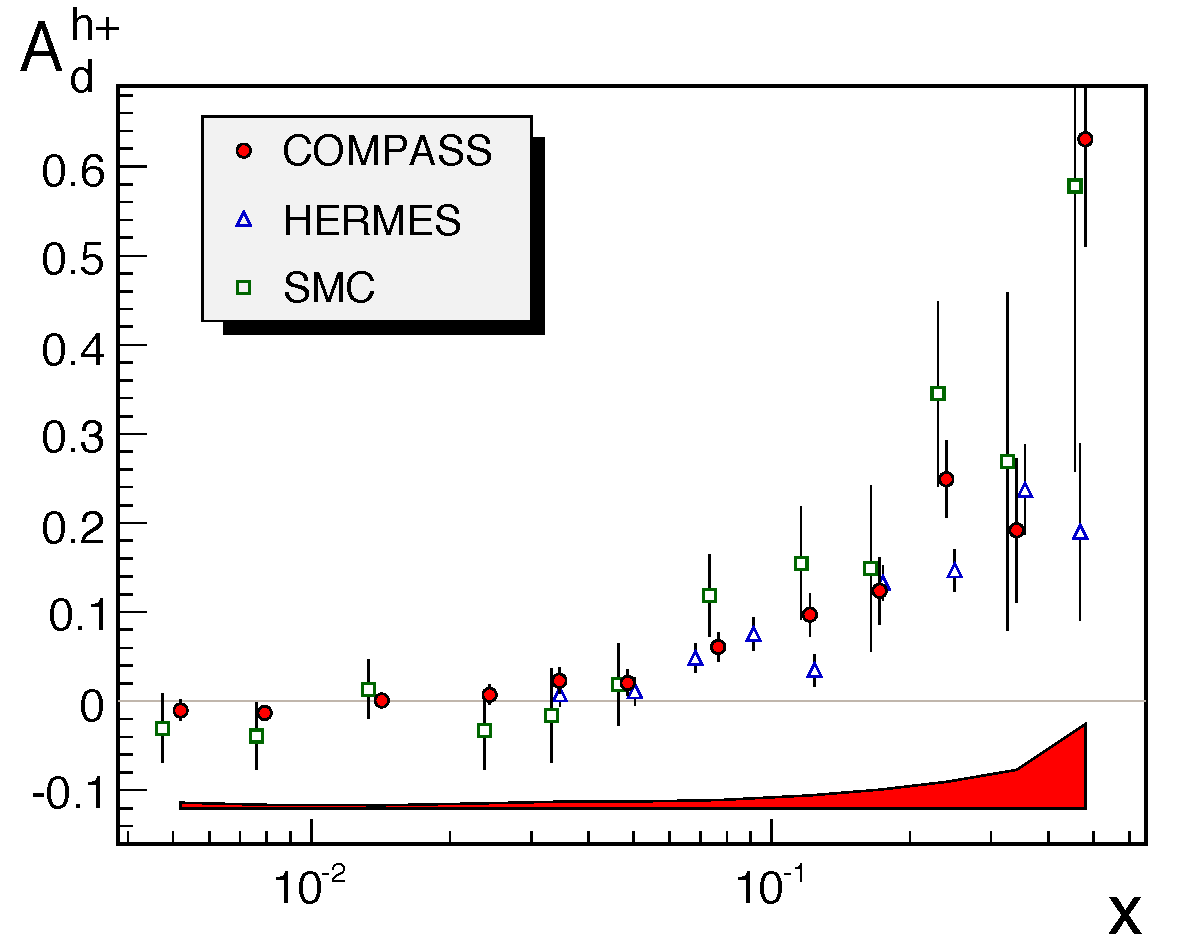
\includegraphics[width=0.48\linewidth]{./figs_xj/compass_apm_proc_12_p.pdf}
    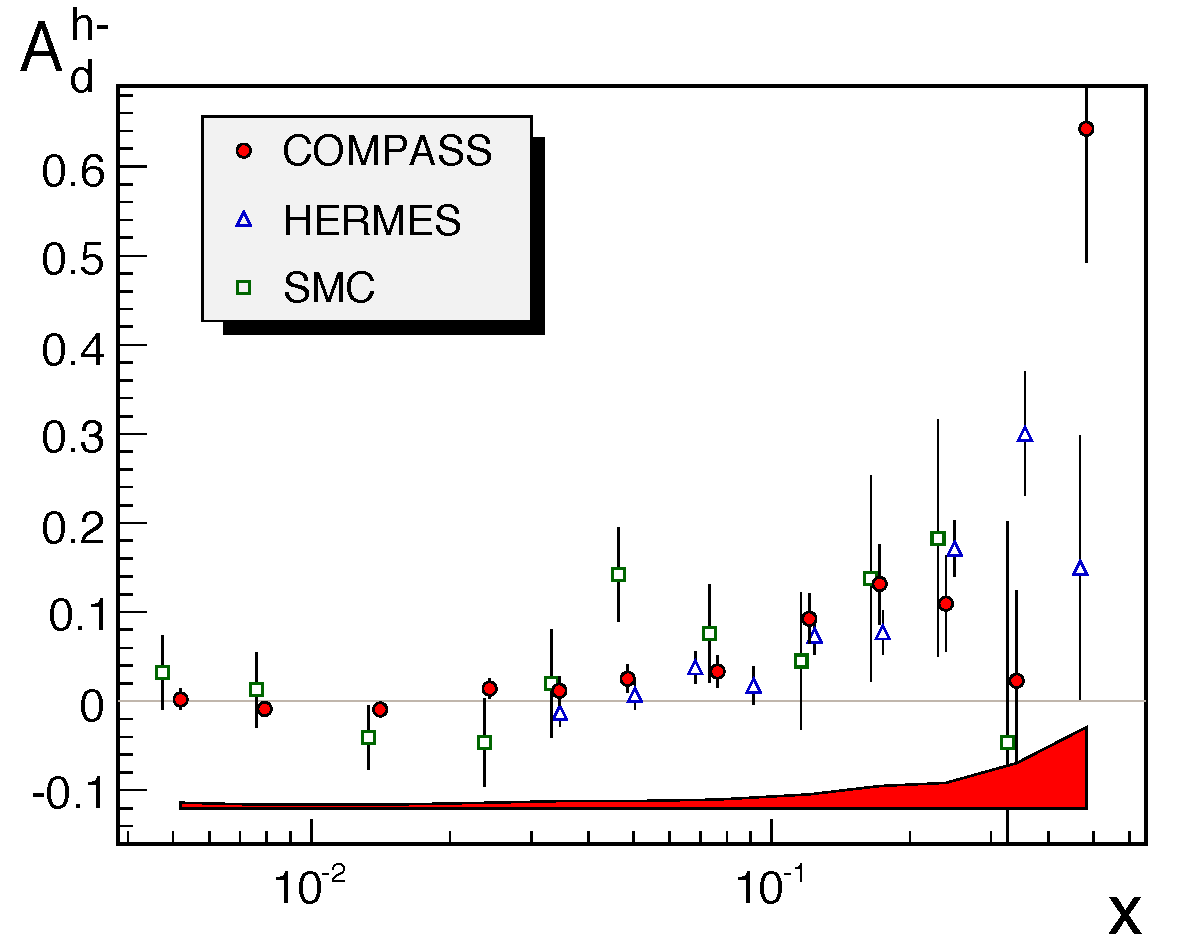
\includegraphics[width=0.48\linewidth]{./figs_xj/compass_apm_proc_12_m.pdf}
\caption{\label{fig:compass1} Hadron asymmetry $A_d^{h^+}$ and $A_d^{h^-}$ measured by COMPASS~\protect\cite{compass2007}, SMC and HERMES.
}
\end{figure}
%-------------------------------------------------------------------------------

\section{NLO global fit to DIS and SIDIS Data}
 The NLO global fit (DSSV2008)~\cite{DSSV2008} to the existing DIS and SIDIS data published up to 2008  are shown in Fig.~\ref{fig:sasnlo}. 
%---------------------------------------------------------------------------------------------
\begin{figure}[htbp]
\vspace{-1.0cm}
  \centering
    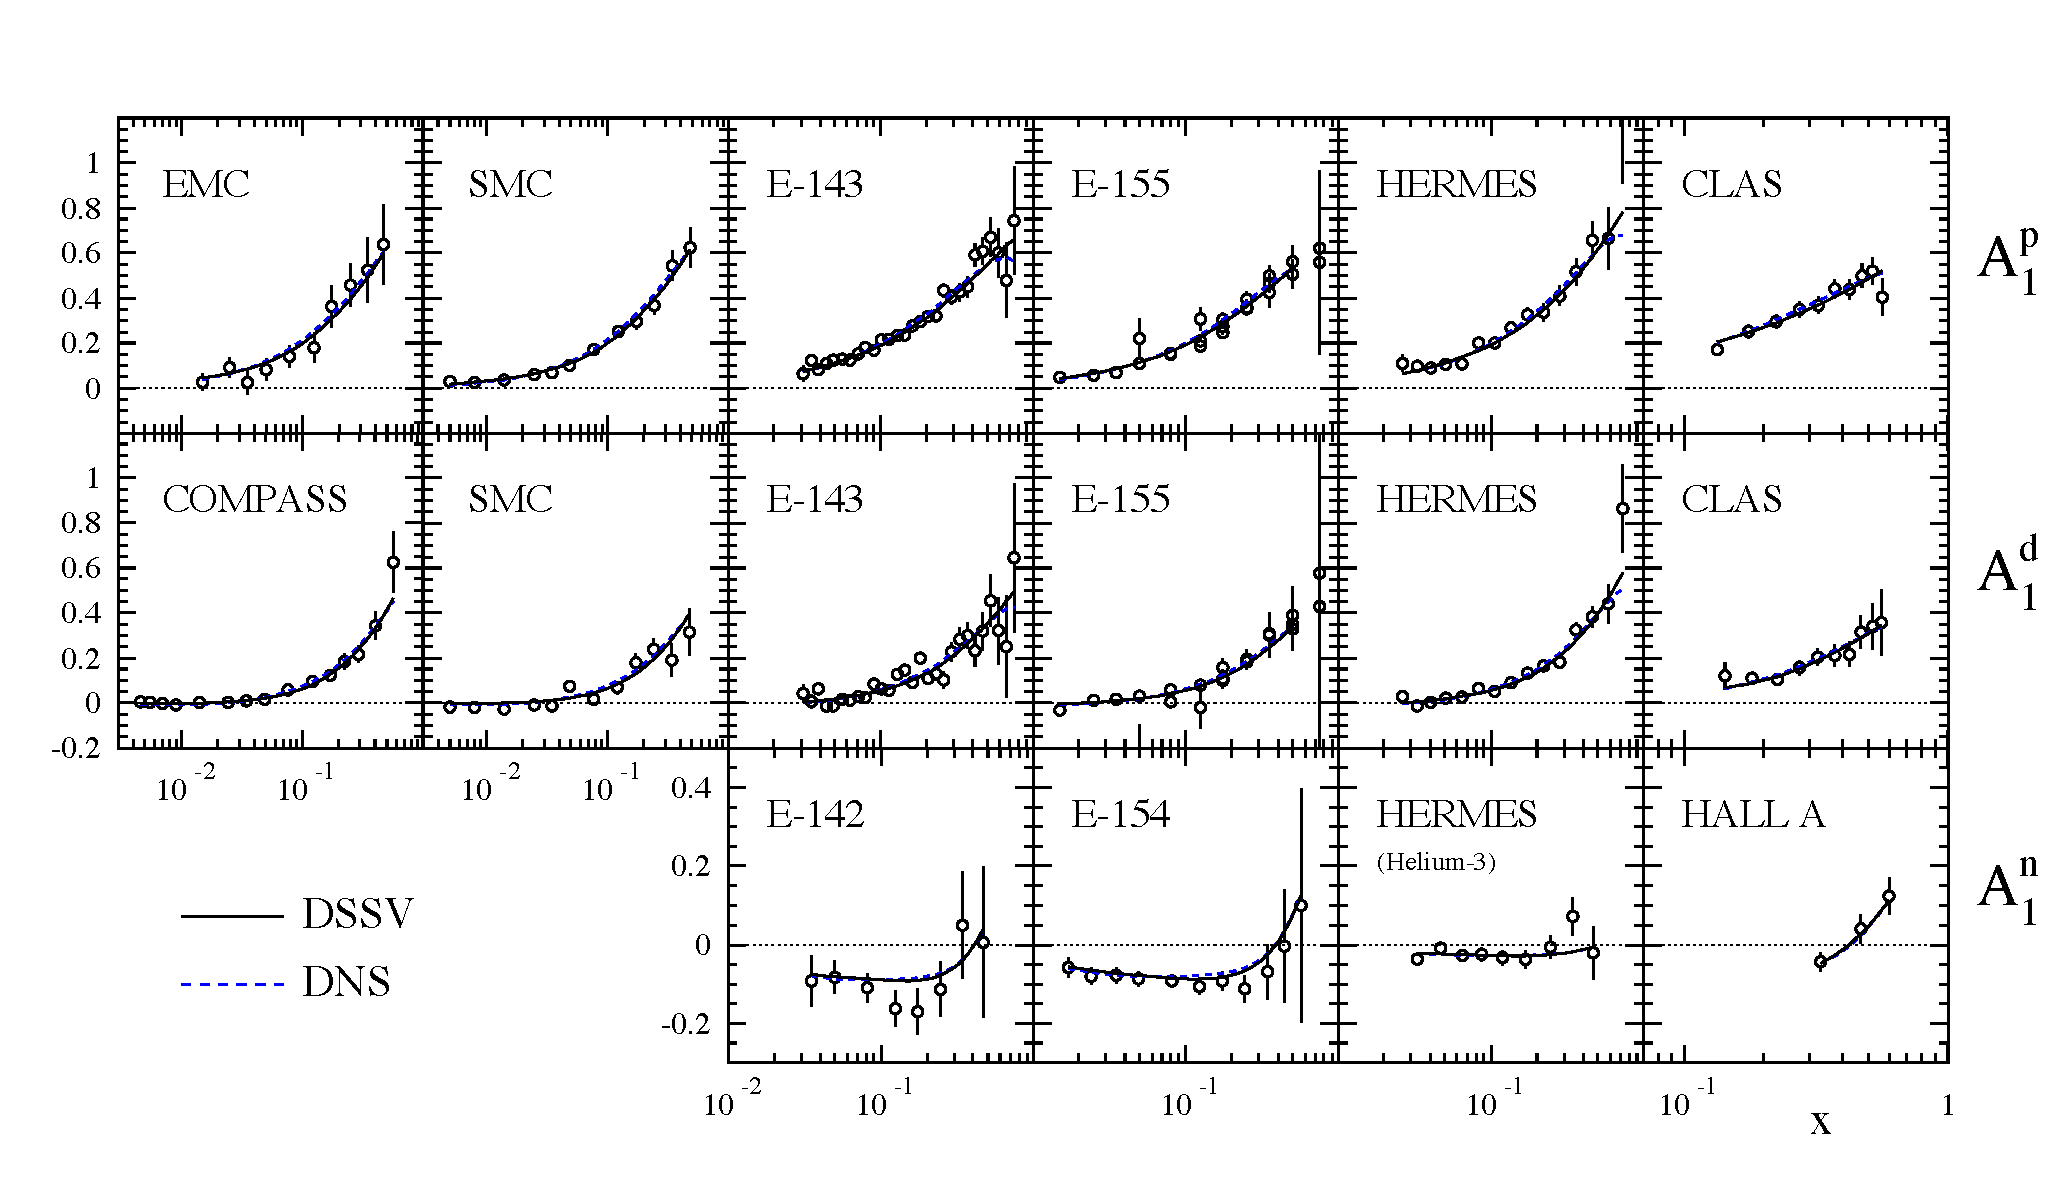
\includegraphics[width=0.90\linewidth]{./figs_xj/sassot_disnlo.pdf} \\
\vspace{-0.2cm}
    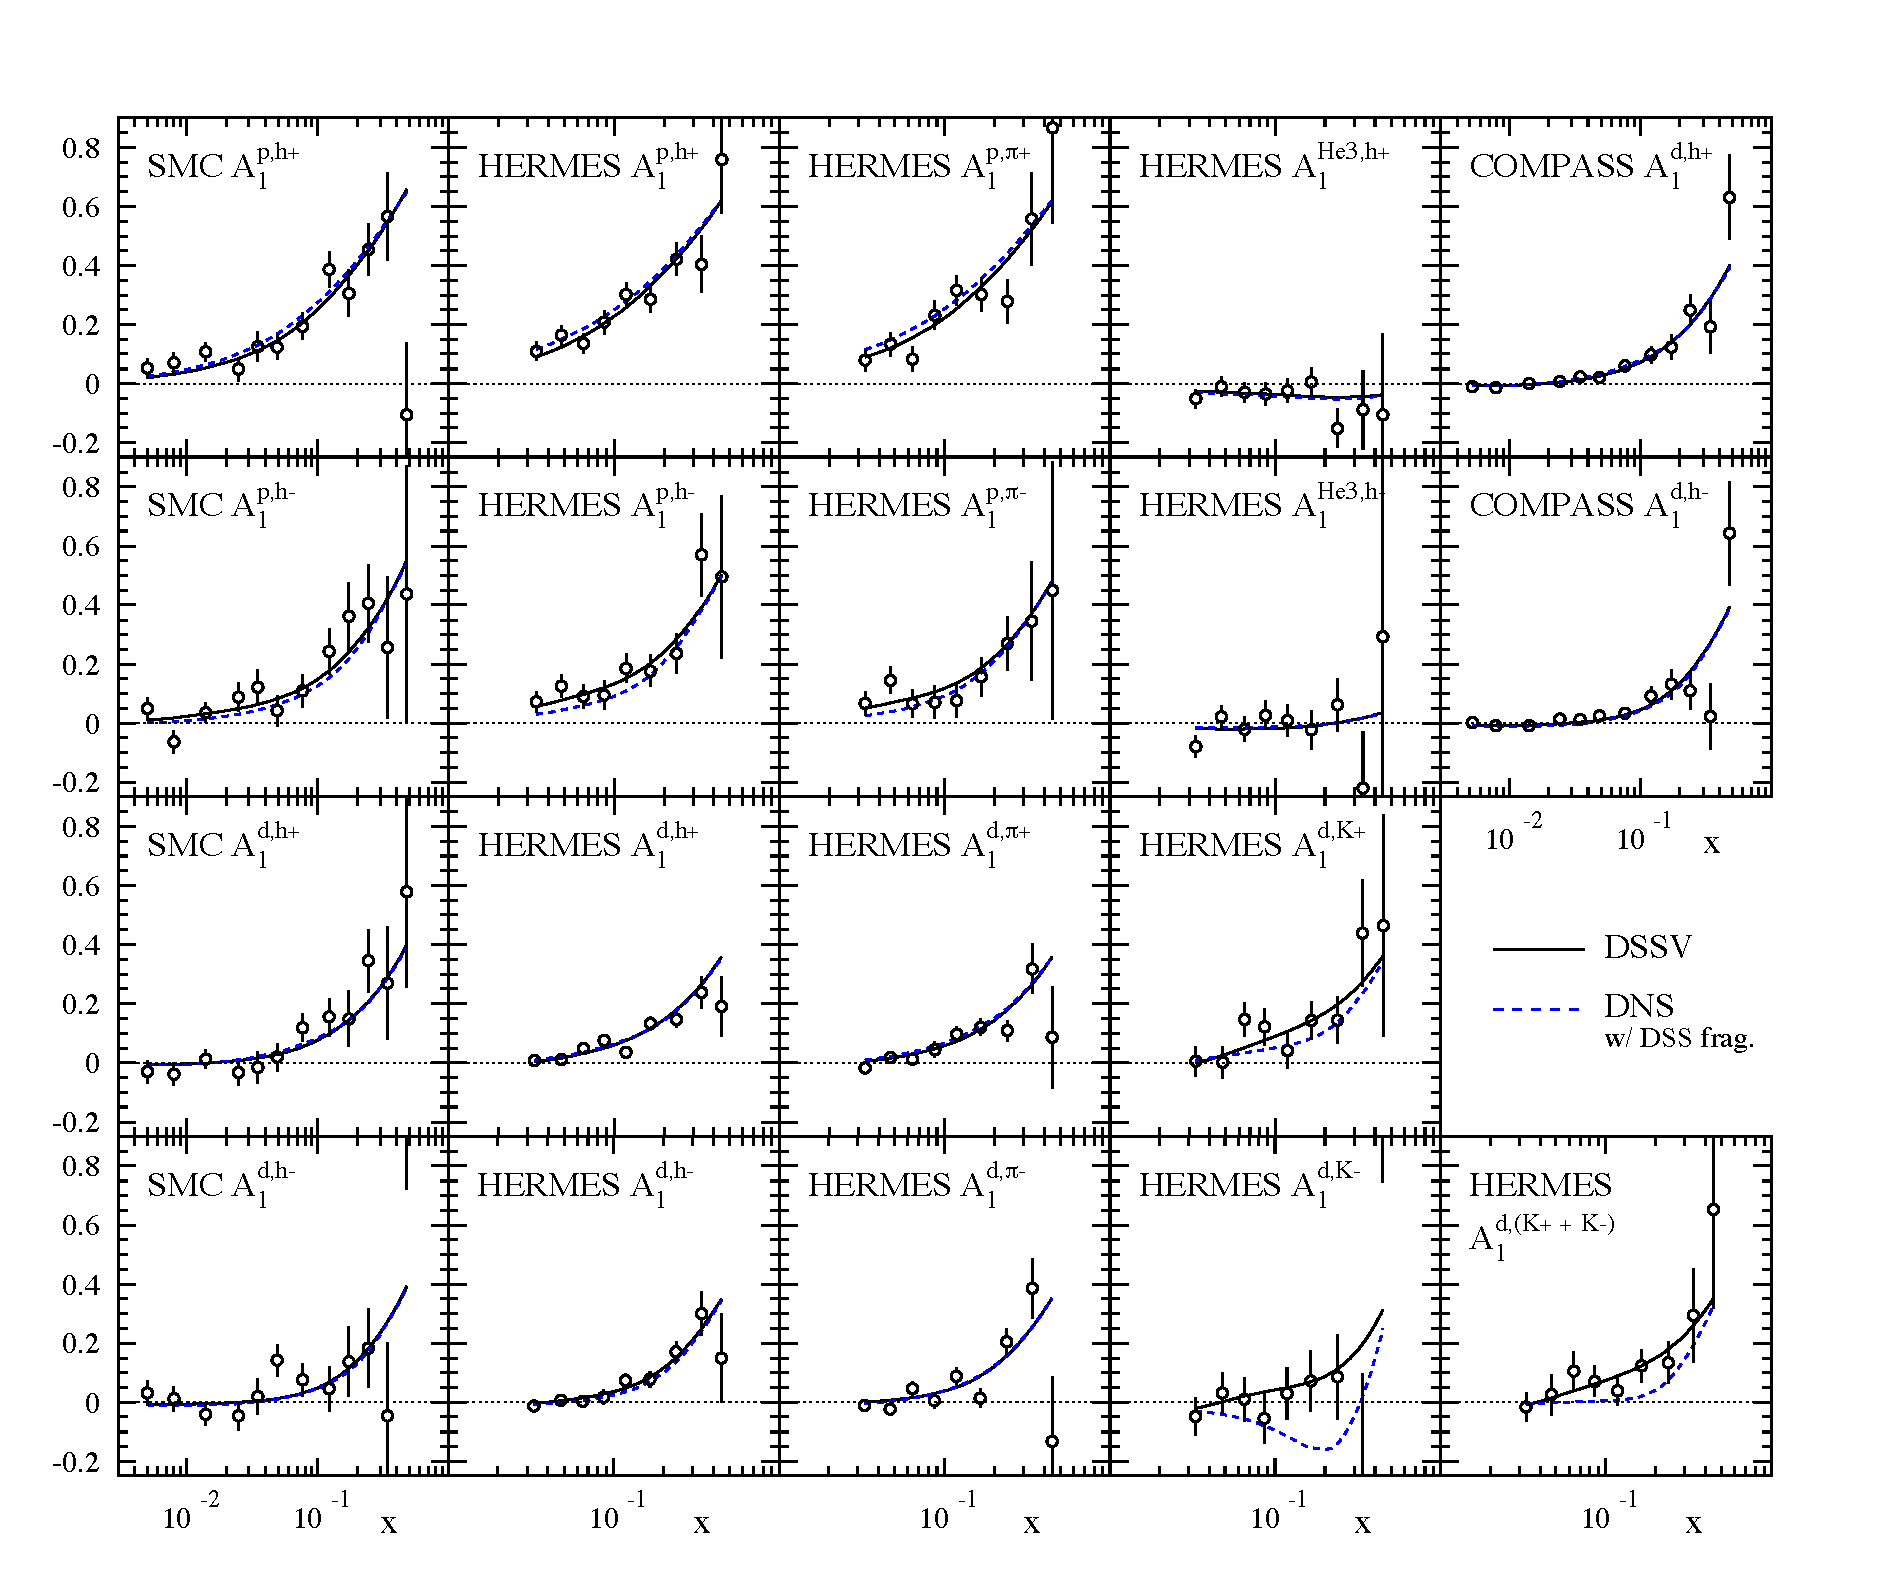
\includegraphics[width=0.90\linewidth]{./figs_xj/sassot_sidisnlo.pdf}
\caption{\label{fig:sasnlo} NLO global fit~\protect\cite{DSSV2008} 
to inclusive DIS data (top) and SIDIS data (bottom). 
}
\end{figure}
%-------------------------------------------------------------------------------

%Formalism and main results.

